\section{Reproducible experiments and their limits}
\label{sec:experiments}

All native comparisons start with the same source triangulation and
normal-coordinate vector.  Source files are hashed before and after the
whole-cut audit.  Every positive native output is replayed by the
existing outer verifier, including the new kernel schema where present.
Raw JSON, complete new packets, commands, logs, and independent finite
checkers accompany the article.  The counts below refer to this fixed
corpus, not a random sample of all knots or all normal surfaces.

\subsection{Native coverage: distinguish the core from the whole cut}

\begin{table}[htbp]
\centering
\begin{tabular}{llrrr}
\toprule
Operation & Corpus & Cases & Canonical & Deferred\\
\midrule
Core certificate & Historical & 106 & 100 & 106\\
Core certificate & Additional interior cases & 14 & 10 & 12\\
\cmidrule(lr){2-5}
& Total & 120 & 110 & 118\\
\midrule
Whole-cut census & Historical & 106 & 92 & 99\\
Whole-cut census & Additional interior cases & 14 & 10 & 12\\
\cmidrule(lr){2-5}
& Total & 120 & 102 & 111\\
\bottomrule
\end{tabular}
\caption{Complete source-authenticated certificates.  All previous
positive cases remain positive.  An inconclusive result is not a
negative manifold or knot verdict.}
\label{tab:coverage}
\end{table}

After the existing dual breadth-first reduction, every historical source
core now peels, and the additional interior corpus has two remaining
core obstructions.  Their greatest stopping residuals contain ten rows
for \code{nested\_1\_4\_6/interior\_links} and four for
\code{interior\_loop/interior\_links}.  The independent stopping checker
validates each residual on reconstructed core occurrences.  The
universal quantifier is over primal forests for that fixed retained
matrix; neither another dual choice nor another move class is excluded.

Whole-cut success is stricter.  The source cores must be recombined with
the parallelity bundles and their annular gluing data.  The full audit
obtains 111 successes rather than 118.  This is why a report of
``106 out of 106'' without saying \emph{cores} would be misleading.

The nine new whole-cut packets are listed in
Table~\ref{tab:new-packets}.  The notation $g^m$ means $m$ components of
genus $g$, not a power in a numerical calculation.

\begin{table}[htbp]
\centering\small
\begin{tabular}{lll}
\toprule
Source identifier & Census & New kernel v3 used?\\
\midrule
\code{pilot/fibonacci\_lst\_04/0} & $1^1,2^1$ & No\\
\code{pilot/fibonacci\_lst\_06/0} & $1^1,2^1$ & No\\
\code{pilot/fibonacci\_lst\_08/0} & $1^1,2^1$ & Yes\\
\code{pilot/fibonacci\_lst\_10/0} & $1^1,2^1$ & Yes\\
\code{pilot/lst\_4\_9/0} & $1^1,2^1$ & No\\
\code{pilot/finite\_trefoil/0} & $2^1$ & No\\
\code{pachner23\_5\_8\_2/mixed} & $0^1,1^2$ & No\\
\code{interior\_loop/empty} & $1^1$ & Yes\\
\code{interior\_loop/boundary\_link} & $0^1,1^1$ & Yes\\
\bottomrule
\end{tabular}
\caption{Nine new complete whole-cut source packets.  Other positive
paths use existing core/absorption schemas with supplied forests.}
\label{tab:new-packets}
\end{table}

There are $102+111=213$ independent positive whole-cut replays in the
paired audit.  The separate Regina literal-cut oracle completes on 113
of the 120 inputs.  It agrees with all 104 deferred positives among
those 113 cases.  The other seven native positives exceed the oracle's
4,096-normal-disc expansion cap; their native certificates still replay,
but no literal comparison is claimed.  No oracle timeout or discrepancy
was observed in this run.

Of the nine remaining deferred refusals, eight contain a component that
the literal oracle identifies as a nonhandlebody.  The remaining example,
\code{pilot/finite\_figureEight/0}, is a union of genus-one and genus-two
handlebodies.  It is an explicit incompleteness witness for the present
whole-cut certificate strategy.  The eight other refusals are consistent
with the oracle but are still only \code{INCONCLUSIVE} in the native API.

\subsection{Finite exhaustive audits}

The exceptional selector was compared against an independent oracle that
enumerates every spanning tree and peels using literal, uncapped integer
column totals.  The oracle imports neither the selector's tree routines
nor its peeling backend.  It independently replays every positive output.

\begin{table}[htbp]
\centering
\begin{tabular}{lr}
\toprule
Finite instance class & Instances\\
\midrule
Exhaustive three-row, two-column cases & 46,656\\
Seeded general weighted cases & 2,000\\
Seeded cycle-compatible column cases & 2,000\\
Additional edge cases & 2\\
\midrule
Total & 50,658\\
Successful trees, independently replayed & 5,183\\
No allowed successful tree & 45,475\\
Mismatches & 0\\
\bottomrule
\end{tabular}
\caption{Standalone finite selector audit.  Random matrices are not
asserted to have native geometric realizations.}
\label{tab:finite-audit}
\end{table}

The exhaustive family has three row edge records chosen from a null
record, a root loop, a nonloop joining two vertices, and a loop at the
other vertex; six matrix entries range over $\{0,1,2\}$.  It therefore has
$4^3 3^6=46{,}656$ instances.  Disconnected graphs test the input rejection
path as well as connected instances testing the theorem.  The audit also
checks partial-partition counts for $u=0,\ldots,6$:
\[
 1,\ 2,\ 5,\ 15,\ 52,\ 203,\ 877,
\]
and two zero-budget cases.  Its recorded runtime is an audit detail, not
evidence for a worst-case exponent.

The deferred primal tests independently enumerate every spanning forest
on 120 seeded small closed-walk instances and compare existence of a
successful forest with full-matrix peeling.  Native tests cover the
strict source gains, loops, repeated bridge traversals, the closed-walk
hypothesis, and rejected certificate mutations.  The geometric family
proof is separate from these finite checks.

\subsection{Regression accounting}

All 1,707 distinct real tests in the restored baseline-plus-patch test
inventory pass across the main run and targeted recovery.  This is not
reported as one clean invocation: the initial sparse checkout omitted
historical fixtures and reference modules.  Its 1,620 reported tests
included eleven failed-import placeholders; there were also 29
fixture-dependent method errors and three failed class setups.

Restoring the required tracked directories resolved those dependencies.
The 24 affected modules contain 174 tests.  Three CLI tests initially
failed in the recovery harness because its working directory did not
propagate to their subprocess import paths; those three passed when run
from the documented \code{fast} directory.  No production edit was needed.
There were 1,580 initial real passes, 174 recovered tests, and 47 overlaps,
giving $1{,}580+174-47=1{,}707$ distinct passes.  A discovery-only inventory
confirms that count and zero loader errors.  All eleven new test methods
are included.  Logs and exact commands retain the unsuccessful
environmental runs as well as the successful recovery.

\subsection{Performance: stronger search does have a local cost}

Final timings were run after test activity finished, with CPython
3.12.14, Regina 7.4, and Linux 6.18.44 on x86-64.  These are measurements
in one runtime environment, not statistically representative performance
claims.  Raw samples and all timer boundaries are supplied.

For the 110 native cores on which both strategies succeed, we precompute
source geometry and the dual reduction, then time nine alternating-order
repeats of 25 corpus passes: 2,750 core-producer calls per measurement.
The median batch time is 116.115 ms for canonical and 161.272 ms for
deferred, a ratio of 1.389.  Thus the stronger core producer is about
39\% slower on this common-success subset.  These timings exclude source
preparation and certificate replay.  They explain the opt-in default;
they do not negate the exact elimination of primal enumeration.

For six common-success whole-cut queries, Table~\ref{tab:whole-timing}
times the complete native producer plus independent replay.  Seven
randomized-order pairs are used per case, followed by three deferred/deferred
A/A pairs.  Short timings show visible variability; both medians and
median paired ratios are retained, which need not equal the ratio of
the two separate medians.

\begin{table}[htbp]
\centering\small
\begin{tabular}{lrrr}
\toprule
Common-success source & Canonical ms & Deferred ms & Paired D/C\\
\midrule
\code{fibonacci\_lst\_01} & 2.066 & 2.317 & 1.104\\
\code{fibonacci\_lst\_03} & 5.073 & 5.075 & 0.989\\
\code{fibonacci\_lst\_05} & 58.498 & 65.774 & 1.017\\
\code{fibonacci\_lst\_07} & 67.588 & 70.509 & 1.045\\
\code{lst\_0\_1} & 14.816 & 16.235 & 1.003\\
\code{lst\_1\_5} & 28.618 & 30.770 & 1.005\\
\bottomrule
\end{tabular}
\caption{Complete native-query medians.  Identifiers abbreviate
\code{pilot/<name>/0}.  A ratio above one favors canonical.}
\label{tab:whole-timing}
\end{table}

For new successes, a canonical refusal is not a comparable successful
operation.  Instead we compare deferred production plus replay with
Regina source construction, explicit cutting, and recognition of every
component, starting from the same raw input.  Table~\ref{tab:oracle-timing}
shows that the native path is slower on five of these six small expanded
inputs.  The trefoil-related cut favors the native path.  These results
support no blanket claim of a faster wall-clock recognizer; the benefits
are a larger certified compressed class and a proved removal of a
search variable.

\begin{table}[htbp]
\centering\small
\begin{tabular}{lrrr}
\toprule
New-success source & Deferred ms & Explicit ms & Paired D/E\\
\midrule
\code{pilot/fibonacci\_lst\_04/0} & 42.258 & 1.963 & 25.880\\
\code{pilot/fibonacci\_lst\_08/0} & 69.602 & 6.593 & 10.720\\
\code{pilot/fibonacci\_lst\_10/0} & 86.238 & 9.897 & 8.650\\
\code{pilot/finite\_trefoil/0} & 5.632 & 28.922 & 0.190\\
\code{interior\_loop/empty} & 3.327 & 0.634 & 5.421\\
\code{interior\_loop/boundary\_link} & 6.791 & 1.081 & 6.278\\
\bottomrule
\end{tabular}
\caption{Same successful whole-cut census query, different operations.
Explicit means Regina's expanded cut and component recognizer.  No
complete knot-diagram recognition is timed.}
\label{tab:oracle-timing}
\end{table}

\subsection{The all-size forest family}

At $h=10$, the specified unpruned lexicographic baseline examines exactly
29,525 forests among 59,049 candidates before its first success.  It took
882.154 ms; deferred core discovery averaged 0.05655 ms over 101 calls.
The theorem, not the timing ratio, establishes the asymptotic separation
from that particular enumeration.  A block-aware algorithm also solves
this family efficiently.

The saved driver separately scales deferred discovery through six sizes,
\[
h=16,64,256,1024,4096,16384,
\]
storing five timings at each size.  Its queue
visits exactly $5h$ incidences, performs no fill updates, and emits $2h$
pivots.  Allocation and cache effects make wall-clock measurements
nonuniform; an indexed linear-work proof is stronger evidence than
fitting a slope to those six points.  The family has a genuine handle
realization, but the benchmark consumes explicit graph walks and does
not authenticate a native triangulation.

\begin{figure}[htbp]
\centering
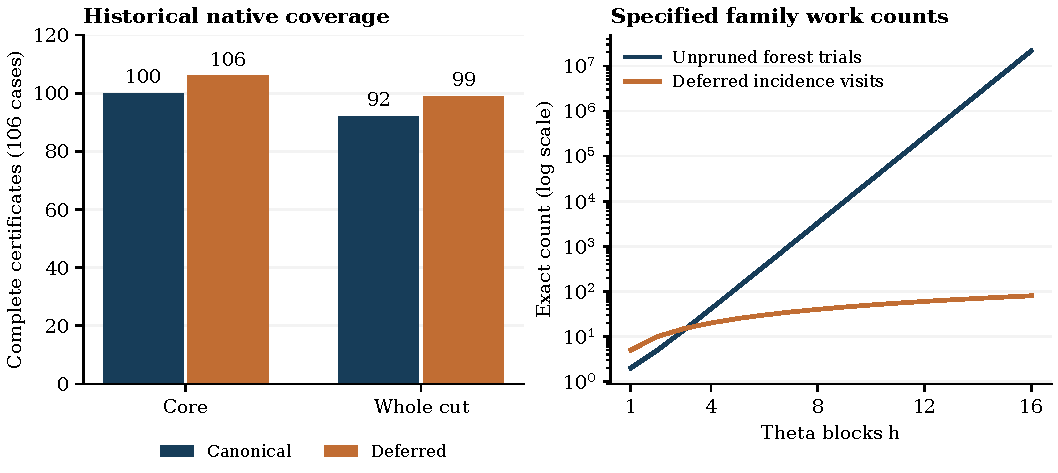
\includegraphics[width=\textwidth]{figures/research_results.pdf}
\caption{Left: exact historical certificate counts, separating cores
from whole cuts.  Right: the proved number of forests tested by the
specified unpruned family enumerator and the number of deferred incidence
visits.  The right panel compares exact work counts of different kinds;
it is not a universal lower bound or a wall-clock speedup chart.}
\label{fig:results}
\end{figure}
\FloatBarrier
